
%------------------------------------------------------------------------------
\section{Entity-Relationship Model (ERM)}
%------------------------------------------------------------------------------

%------------------------------------------------------------------------------
\begin{frame}{Das Entity-Relationship Model nach Peter Chen}
\metroset{block=fill}
\begin{block}{\cite[9]{chen1976}}
    \begin{quote}
        The entity-relationship model can be used as a basis for unification of different views of data: the network model, the relational model, and the entity set model.~
    \end{quote}
\end{block}
\begin{block}{\cite[10]{chen1976}}
    \begin{quote}
        \lbrack{}Der Text\rbrack{} analyzes the network model, the relational model, and the entity set model, and describes how they may be derived from the entity relationship model.~
    \end{quote}
\end{block}
\begin{block}{\cite[19]{chen1976}}
    \begin{quote}
        \lbrack{}Der Text stellt vor:\rbrack{} a diagrammatic technique for exhibiting entities and relationships: the entity-relationship diagram.~%\parencite[19]{chen1976}
    \end{quote}
\end{block}
$\to$ \alert{Konzeptuelles Modell}

\end{frame}

%------------------------------------------------------------------------------
\begin{frame}{ER-Begriffe~\parencite[9--12]{chen1976}}
    % ----------------------------------------------
  \begin{columns}[T,onlytextwidth]
  \metroset{block=fill}
    \column{0.55\textwidth}\footnotesize
      \begin{block}{Entität (Entity)}
       An entity is a „thing“ which can be distinctly identified. A specific person, company, or event is an example of en entity.
      \end{block}

      \begin{alertblock}{Beziehung (Relationship)}
        A relationship is an association among entites. For instance, „father-son“ is a relationship between two „person“ enitities.
      \end{alertblock}

      \begin{exampleblock}{Entitätsmenge (Entity Set)}
        Alle Entitäten derselben Entitätsmenge haben dieselben Eigenschaften (properties). 
        
        „Entities are classified into different entity sets such as EMPLOYEE, PROJECT, and DEPARTMENT.“
      \end{exampleblock}

    % ----------------------------------------------

    \column{0.4\textwidth}

      \metroset{block=fill}

      \begin{block}{ER-Modell-Bestandteile}
      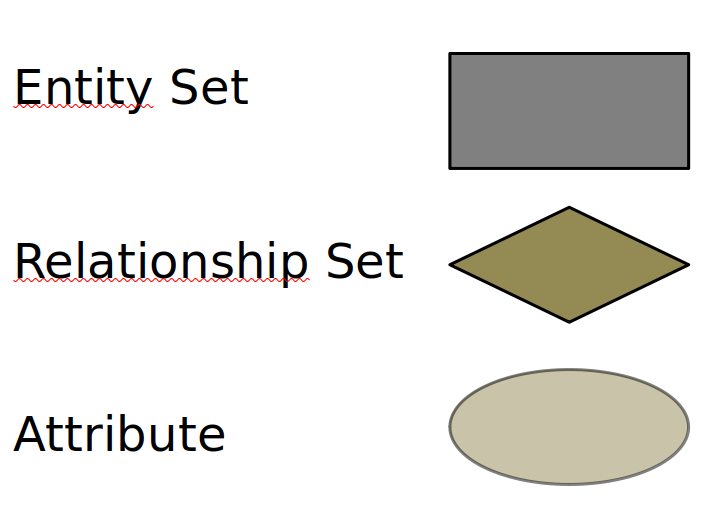
\includegraphics[width=0.9\textwidth]{img/er-modell.png}
      \end{block}
      
      \begin{block}{ER-Modell-Bestandteile}
      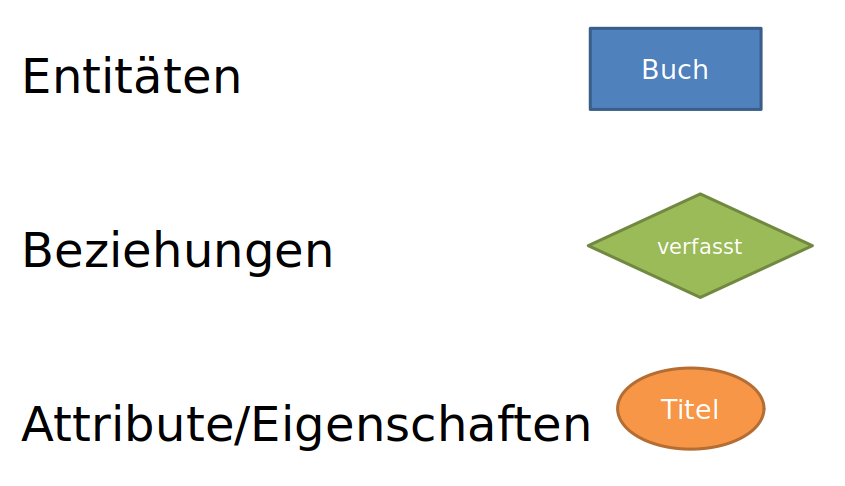
\includegraphics[width=0.9\textwidth]{img/er-bsp2.png}
      \end{block}
  \end{columns}

\end{frame}

%------------------------------------------------------------------------------
\begin{frame}{ER-Begriffe~\parencite[9--12]{chen1976}}
    % ----------------------------------------------
  \begin{columns}[T,onlytextwidth]
  \metroset{block=fill}
    \column{0.48\textwidth}\footnotesize
      \begin{exampleblock}{Menge von Beziehungen (Relationship Set)}
        Gleiche Beziehungen zwischen Entitäten, die jeweils aus derselben Entitätsmenge stammen, lassen sich in einer Menge von Beziehungen zusammenfassen. 
      \end{exampleblock}

    % ----------------------------------------------

    \column{0.48\textwidth}

      \metroset{block=fill}
      \begin{block}{Rolle (Role)} \footnotesize
        The role of an entity in a relationship is the function that it performs in the relationship.
      \end{block}
      
      \begin{alertblock}{Eigenschaften (Properties)}\footnotesize
        Mithilfe von Eigenschaften lassen sich Entitäten (Entities) und Beziehungen (Relationships) beschreiben. 
      \end{alertblock}
  \end{columns}
  \begin{center}
      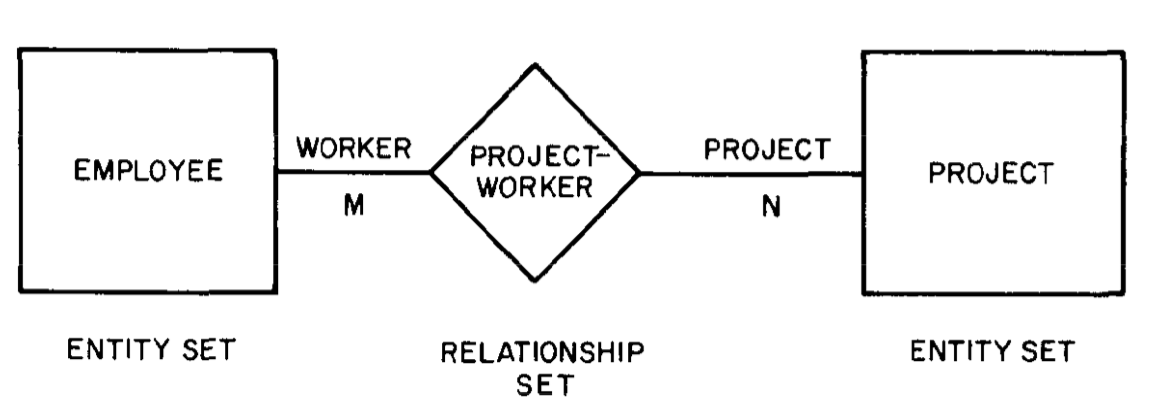
\includegraphics[width=0.6\textwidth]{img/er-bsp.png}
  \end{center}
\end{frame}

%------------------------------------------------------------------------------
\begin{frame}{Attribut-Wert-Paare und Primary Keys}
    Eigenschaften (Properties) werden stets durch eine Kombination von Attribut und Wert ausgedrückt. Beispiel: 
    \begin{enumerate}
        \item Der Stift ist blau = Die Entität `Stift' hat das Attribut „Farbe“ mit dem Attributwert „blau“ 
        \item Der Stift ist rot = Die Entität `Stift' hat das Attribut „Farbe“ mit dem Attributwert „rot“
    \end{enumerate}

\metroset{block=fill}
\begin{exampleblock}{Primary Key: Identifizierende Eigenschaften}
Entitäten und Beziehungen lassen sich über den Wert eines oder mehrerer Attribute identifizieren. 
Das oder die identifizierenden Attribute werden als Primary Key bezeichnet.
\end{exampleblock}
\end{frame}
%------------------------------------------------------------------------------
\begin{frame}[allowframebreaks,fragile]{Beispiel ER-Modell für ein Buch}
\begin{comment}
    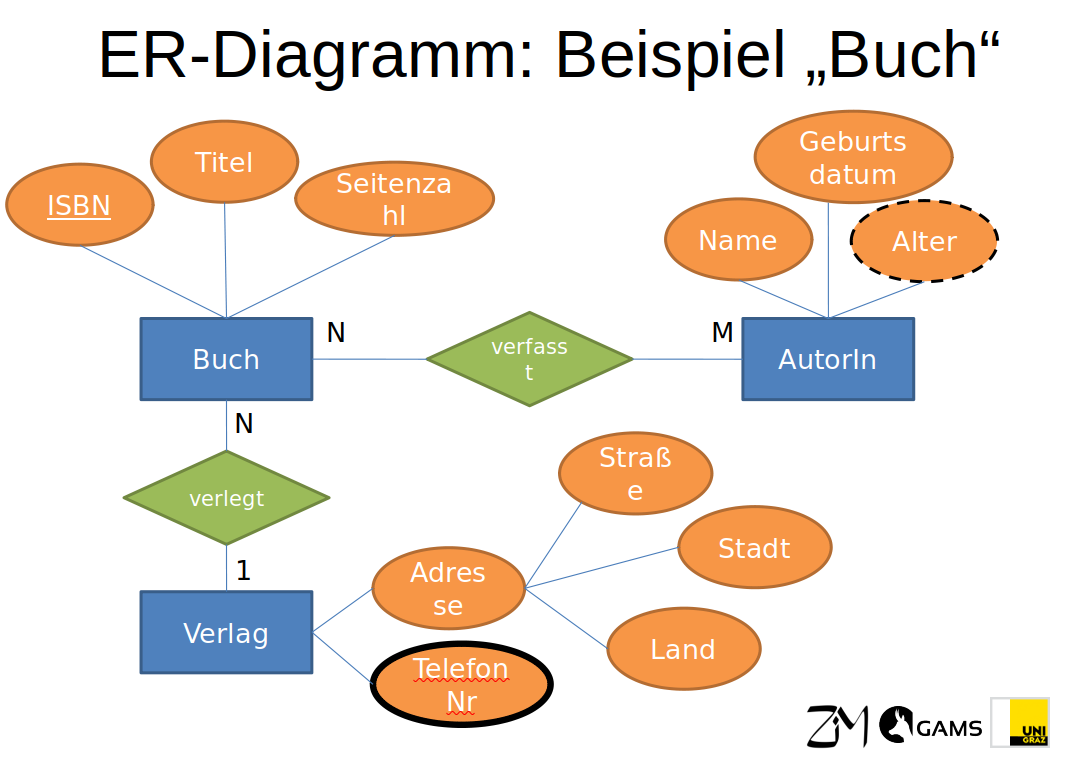
\includegraphics[width=0.9\textwidth]{img/er-bsp3.png} 
    
    \framebreak
\end{comment}

\footnotesize
\begin{tikzpicture}[node distance=5.5em]
%--------------------
% the book
%--------------------
\node[entity](book){Book};
\node[attribute](isbn)[left of=book]{\key{ISBN}} edge(book);
\node[attribute](title)[above left of=book]{title} edge(book);
\node[attribute](pagenr)[above of=book]{nr. of pages} edge(book);

%--------------------
% published by publisher
%--------------------
\node[relationship](published)[below of=book, yshift =-2em]{published} edge node[above right]{N}(book);
\node[entity](publisher)[below of=published, yshift =-2em]{publisher} edge node[above right]{1}(published);
\node[attribute](tid)[left of=publisher]{\key{ID}} edge(publisher);
\node[attribute](tname)[right of=publisher]{Name} edge(publisher);
\node[attribute](address)[above right of=publisher]{address} edge(publisher);
\node[attribute](street)[above right of=address]{Street} edge(address);
\node[attribute](city)[right of=address]{City} edge(address);
\node[multi attribute](phonenr)[below right of=publisher]{phone number} edge(publisher);

%--------------------
% written by author
%--------------------
\node[relationship](written)[right of=  book, xshift =3em]{written} edge node[above right]{N}(book);
\node[entity](author)[right of= written, xshift =3em]{author} edge node[above right]{M}(written);
\node[attribute](birthday)[above  of=author]{birthday} edge(author);
\node[attribute](name)[above right of=author]{name} edge(author);
\node[derived attribute](age)[right of=author]{Age} edge(author);
\end{tikzpicture}

\end{frame}


%------------------------------------------------------------------------------
\begin{frame}[fragile]{Beispiele}
\metroset{block=fill}
\begin{block}{Entitäten: Unikurs}
    \begin{itemize}
        \item \textbf{Entitäten:} Kurs, Dozent:in, Studierende, Raum
        \item \textbf{Attribute:} Kurs (Nr, Titel), Dozent:in (Name), Studierende (Name, Matrikelnummer, Studium, Fach), Raum (Nr, Gebäude, Sitzplätze)
        \item \textbf{Relationen:}
        \begin{itemize}
            \item Ein Kurs wird abgehalten von Dozent:in.
            \item Er findet in einem Raum statt.
            \item Die Studierenden nehmen am Kurs teil.
        \end{itemize}
    \end{itemize}
\end{block}

\begin{block}{CSV: Geburtsort}\scriptsize
\begin{verbatim}
    "Name","Address","Description","Longitude","Latitude"
    "Vorname Nachname","Teststr. 1, PLZ","Geburtsort","7.018242","50.678667"
\end{verbatim}
\end{block}
\end{frame}


%------------------------------------------------------------------------------
\begin{frame}[allowframebreaks]{(Materialien für die) Hausübung}
\metroset{block=fill}
\begin{exampleblock}{Ressourcen}
    \begin{itemize}\footnotesize
        \item \href{https://erdplus.com/standalone}{Tool zum Entity-Relationship-Modelle erstellen}
        \item \href{https://www.geeksforgeeks.org/introduction-of-er-model/}{GeeksforGeeks-Tutorial/Intro to ER Models}
        \item \href{https://geobrowser.de.dariah.eu/}{DARIAH Geobrowser}

    \end{itemize}
\end{exampleblock}

\begin{alertblock}{Angabe HÜ ER-Model}
    \begin{enumerate}\footnotesize
        \item Konzipieren und visualisieren Sie das Model Ihres Originals (Attributklasse) mithilfe des Entity-Relationship-Diagramms. (z.B. ERDplus siehe oben)
        \item Exportieren Sie ihr Diagramm als Bild und laden es auf Moodle hoch.
        \item Bei Problemen können Sie sich auch gegenseitig im Hilfe-Forum unterstützen.
        %\item Schauen Sie sich das Thema `Kardinalität' an bzw. erarbeiten es sich aus den Unterlagen und bauen Sie es in Ihr Modell ein. 
    \end{enumerate}
\end{alertblock}
\end{frame}

%------------------------------------------------------------------------------
%\begin{frame}[standout]
%    \alert{Lektüre} auf nächste Einheit: \\
%    Chen, ER-Modelle 
%\end{frame}

%\section{ER-Modelle (Wiederholung und Fortsetzung)}
\begin{frame}[allowframebreaks]{Kardinalitäten}
\metroset{block=fill}
    "Kardinalität" =  Anzahl der an einer Beziehung beteiligten Entitäten
    Dabei stehen \textit{n} und \textit{m} für eine beliebig hohe Anzahl.

\begin{block}{Typen von Relationen}
 \textbf{1:1} $\to$ Es gibt genau je eine Entität, die an der Beziehung beteiligt ist.
 
 \textbf{1:n} $\to$ Für jede Entität auf der 1-Seite der Beziehung kann es beliebig viele Entitäten auf der n-Seite geben.
 
 \textbf{n:m} $\to$ Für jede Entität auf der n-Seite der Beziehung kann es beliebig viel Entitäten auf der m-Seite geben und umgekehrt.
\end{block}

\begin{center}
  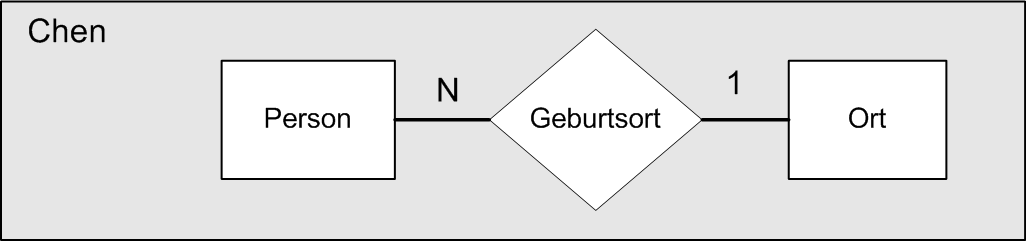
\includegraphics[width=0.7\textwidth]{img/ERD_Darstellungen_Chen.png}
\end{center}

\framebreak
\begin{block}{Minimale Kardinalitäten}
\textbf{0} $\to$ Es muß keine Entität auf dieser Seite der Beziehung geben. (=\textit{optional})

\textbf{1} $\to$ Es muß mindestens eine Entitäten auf dieser Seite der Beziehung geben. (=\textit{verpflichtend})
\end{block}

\begin{center}
    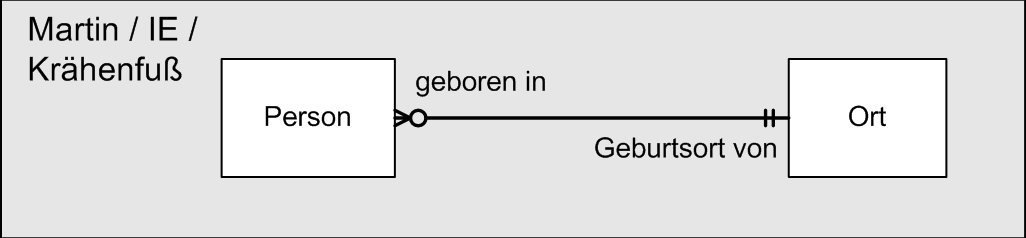
\includegraphics[width=0.7\textwidth]{img/ERD_Darstellungen_Crowfoot.png}
    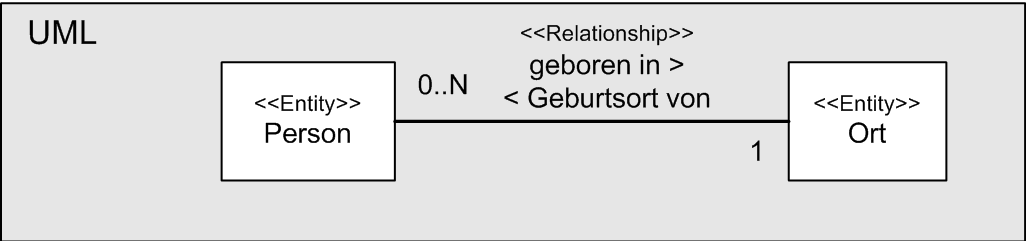
\includegraphics[width=0.7\textwidth]{img/ERD_Darstellungen_UML.png}
\end{center}

\end{frame}

%------------------------------------------------------------------------------
\begin {comment}
\begin{frame}{Wiederholung: ER-Begriffe~\parencite[9--12]{chen1976}}
    % ----------------------------------------------
  \begin{columns}[T,onlytextwidth]
  \metroset{block=fill}
    \column{0.55\textwidth}\footnotesize
      \begin{block}{Entität (Entity)}
       An entity is a „thing“ which can be distinctly identified. A specific person, company, or event is an example of en entity.
      \end{block}

      \begin{alertblock}{Beziehung (Relationship)}
        A relationship is an association among entites. For instance, „father-son“ is a relationship between two „person“ enitities.
      \end{alertblock}

      \begin{exampleblock}{Entitätsmenge (Entity Set)}
        Alle Entitäten derselben Entitätsmenge haben dieselben Eigenschaften (properties). 
        
        „Entities are classified into different entity sets such as EMPLOYEE, PROJECT, and DEPARTMENT.“
      \end{exampleblock}

    % ----------------------------------------------

    \column{0.4\textwidth}

      \metroset{block=fill}

      \begin{block}{ER-Modell-Bestandteile}
      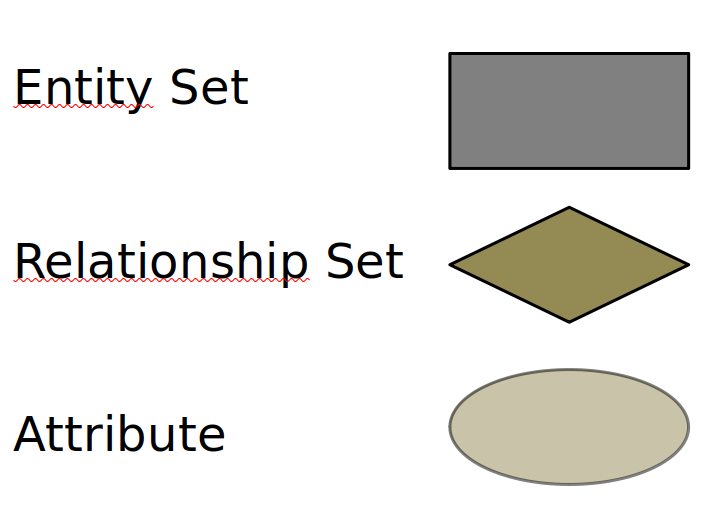
\includegraphics[width=0.9\textwidth]{img/er-modell.png}
      \end{block}
      
      \begin{block}{ER-Modell-Bestandteile}
      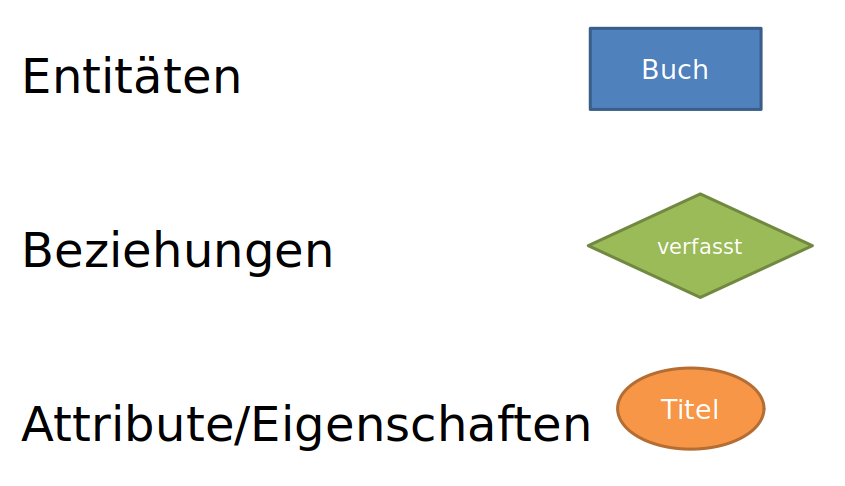
\includegraphics[width=0.9\textwidth]{img/er-bsp2.png}
      \end{block}
  \end{columns}

\end{frame}
\end{comment}

%------------------------------------------------------------------------------
\begin{frame}[allowframebreaks]{ER erweitert}
    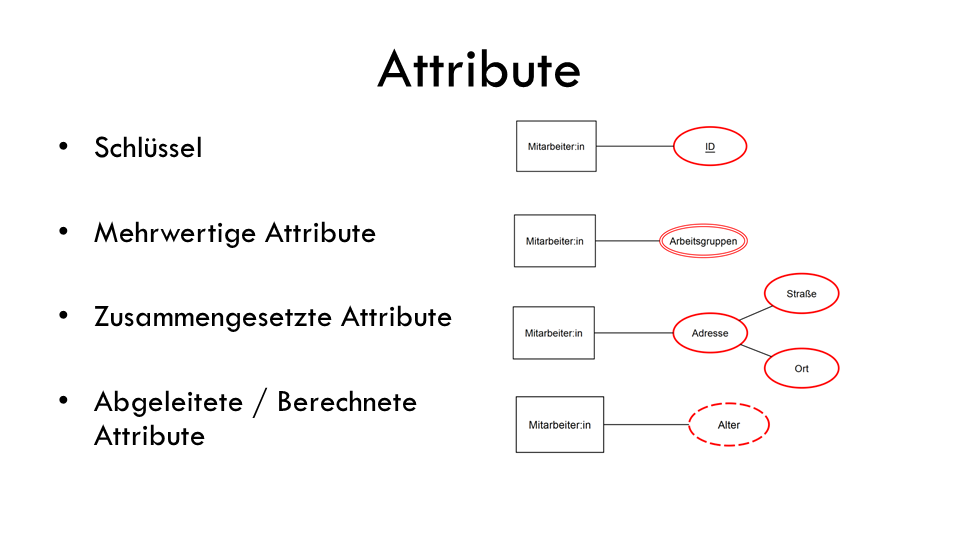
\includegraphics[width=\textwidth]{img/attribute.png}
\end{frame}



%\begin{comment}
\begin{frame}[allowframebreaks]{ER erweitert}
    \begin{itemize}
        \item \textbf{identifizierende Attribute (``Schlüssel``)}: Innerhalb der Entitätsklasse gibt es die Werte dieses Attributs nur genau einmal. Sie können damit die einzelne Entität identifizieren.
        \item \textbf{Mehrwertige Attribute}: Attribute, die mehr als einen Wert enthalten können.
        \item \textbf{abgeleitete Attribute}: Attribute, die sich aus einem anderen Attribut berechnen.
        \item \textbf{zusammengesetzte Attribute}: Attribute, die aus mehreren Teilen bestehen.
    \end{itemize}
    \begin{itemize}
        %\item \textbf{Attribute von Beziehungen}: Auch Beziehungen können Attribute haben.
        \item \textbf{n-äre Beziehungen}: ein Relationship-Set kann prinzipiell mehrere Entity-Sets mit einander verbinden.
        \item \textbf{Schwache Entität}: Kann nur existieren, wenn eine Relation zu einer anderen Entity existiert (Raum in Gebäude), Schlüssel ist abhängig vom Schlüssel einer Relationship (Chen-Notation: Doppelter Rand). Besitzen keine Eigenschaften, anhand derer man sie identifizieren könnte (besitzen keinen Primary Key). Sie werden nur über die Beziehung der schwachen Entität zu einer starken Entität identifiziert. Beispiel: der Angehörige eines Mitarbeiters eines Unternehmens
    \end{itemize}
\end{frame}
%\end{comment}

%-------------------------------------------------
    
\begin{frame}{n-äre Beziehungen}
\begin{center}
    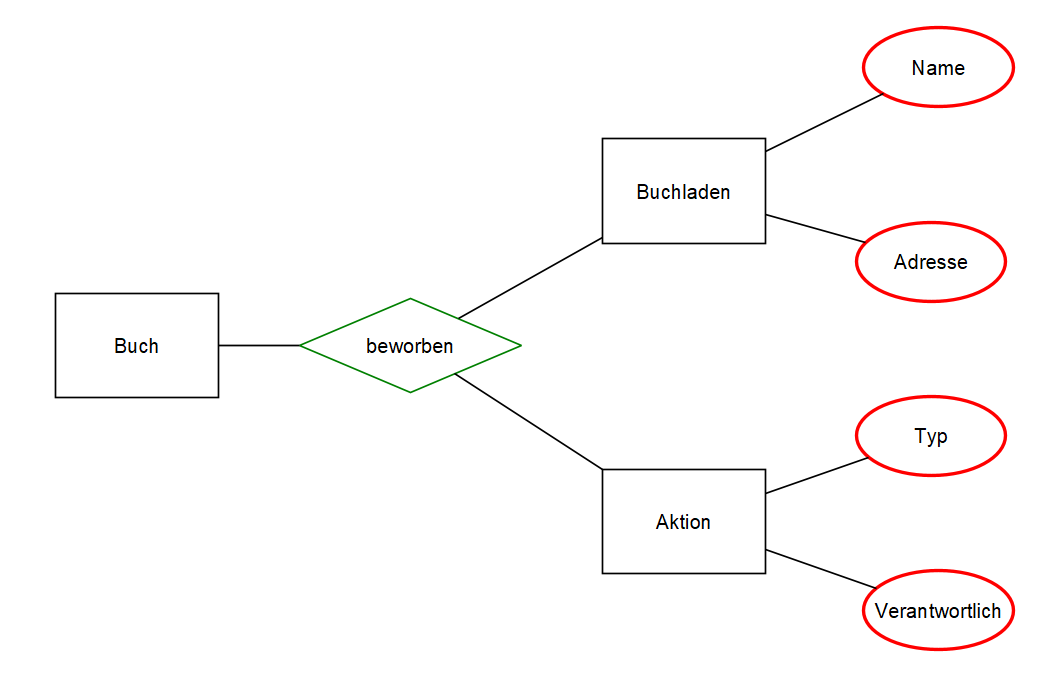
\includegraphics[width=0.9\textwidth]{img/n-ary-relationship.png}
\end{center}    
\end{frame}


%------------------------------------------------------------------------------
\begin{frame}{Übung ER-Modell}
    % ----------------------------------------------
  \begin{columns}%[T,onlytextwidth]
  \metroset{block=fill}
    \column{0.4\textwidth}\footnotesize
    \begin{block}{Eine Kurseinheit einer Lehrveranstaltung}
    Eine Kurseinheit besteht aus folgenden Enitäten:
    \begin{enumerate}
        \item Studierende
        \item Lehrende
        \item Sitzplatz
        \item Kursraum
        \item Gebäude
    \end{enumerate}
    \end{block}

    % ----------------------------------------------

    \column{0.55\textwidth}
      \metroset{block=fill}\footnotesize
      \begin{exampleblock}{Übung}
      \begin{enumerate}
          \item Mit welchen Attributen lassen sich diese Entitäten beschreiben?
          \item Anhand welcher Attribute lassen sich die Entitäten jeweils identifizieren?
          \item Welche Beziehungen existieren zwischen den Entitäten?
      \end{enumerate}
      $\to$ bezogen auf normalen Präsenzunterricht
      \end{exampleblock}
      \begin{exampleblock}{Übung 2}
      Wie müsste man das jetzt umändern, um auch Distance Learning einzukalkulieren?
      \end{exampleblock}
      \footnotesize
      $\to$ Übung in Gruppen. Erstellen Sie, wenn möglich, eine Zeichnung / einen Screenshot der Resultate, der dann vorgestellt wird.
  \end{columns}

\end{frame}


%------------------------------------------------------------------------------
\begin{frame}{Musterlösung Kurseinheit als ER}
    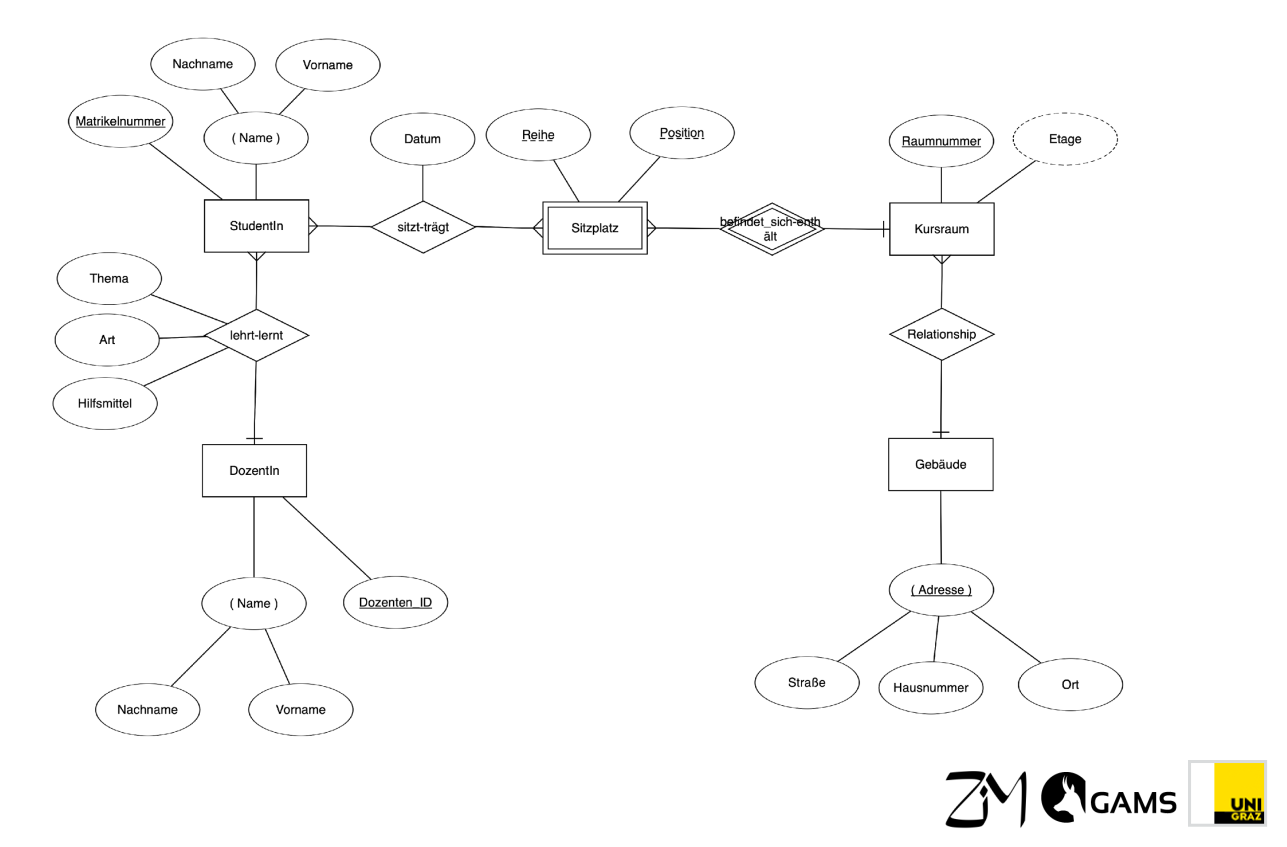
\includegraphics[width=\textwidth]{img/wdh-er-kursmodellierung.png}
\end{frame}


\subsection{ERM -- Tabellen und Relationen}
%------------------------------------------------------------------------------

%------------------------------------------------------------------------------
\begin{frame}{Von ER zur Tabelle?}
    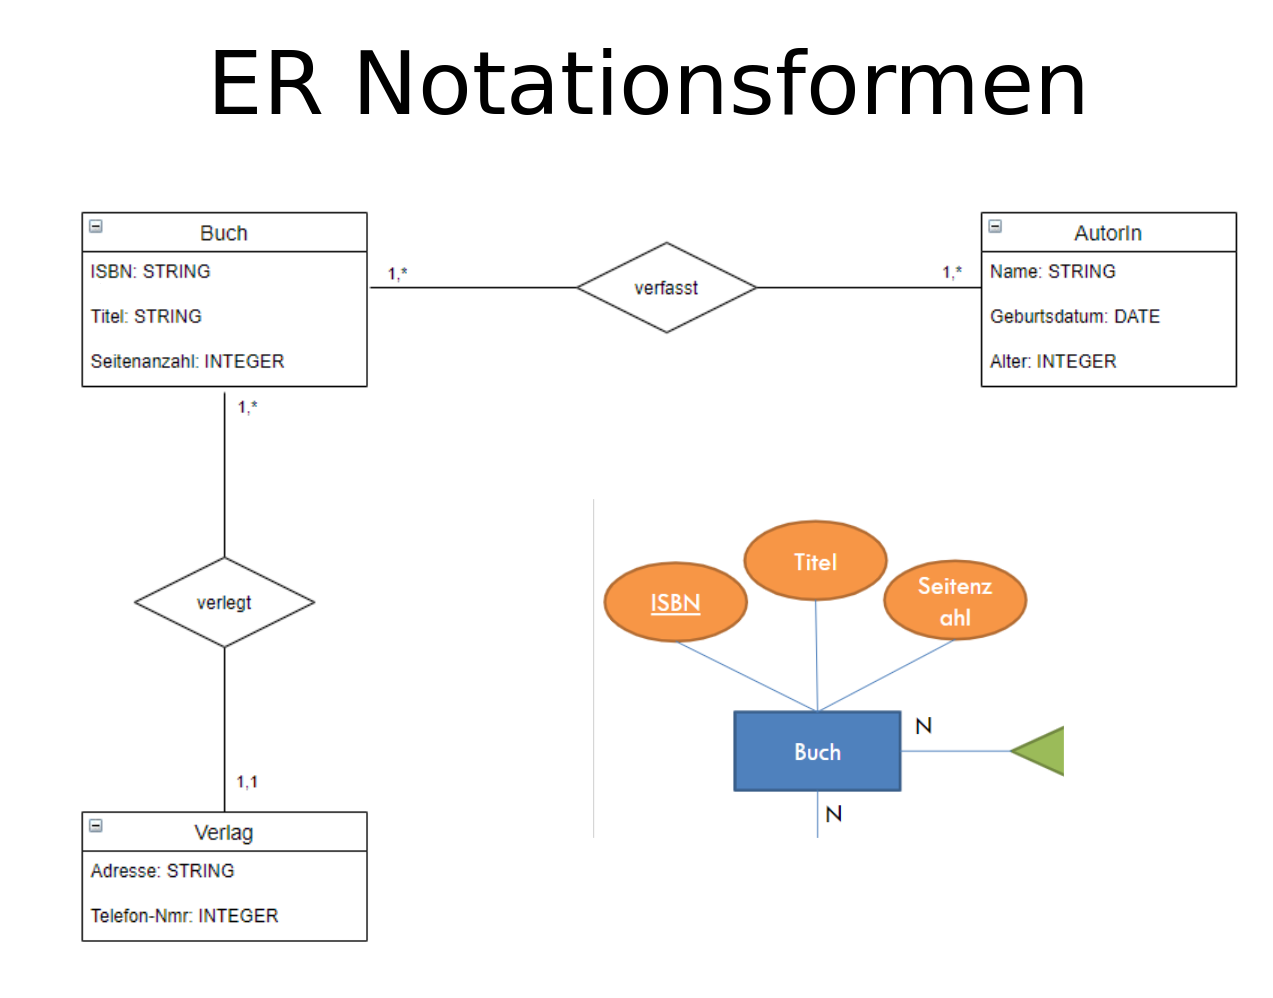
\includegraphics[width=\textwidth]{img/er-notation-buch.png}
\end{frame}

%------------------------------------------------------------------------------
\begin{frame}{Repräsentation von ER-Modellen als Tabellen}
    % ----------------------------------------------
  \begin{columns}[T,onlytextwidth]
  \metroset{block=fill}
    \column{0.4\textwidth}\footnotesize
    \begin{block}{Repräsentation als Tabellen}
    Entitäten und deren Beziehungen können als Tabellen repräsentiert werden. \\
    Die Attribute sind dann die Spalten
    \end{block}

    % ----------------------------------------------

    \column{0.55\textwidth}
      \metroset{block=fill}
      \begin{exampleblock}{Umgang mit Kardinalitäten}
      \begin{enumerate}\small
          \item Gleiches Buch aber mehrere Autoren? (Wieso nicht einfach als Attribut?)
          \item Gleiches Buch mehrere Genre? (Entität oder Attribut)
          \item Wie würde ich den Inhalt eines Buches modellieren?
      \end{enumerate} \small
      %$\to$ diese Leitfragen bitte in der Lektüre-Diskussion später auch beachten (beim Thema Kardinatlität)
      \end{exampleblock}

  \end{columns}
\end{frame}

%------------------------------------------------------------------------------
\begin{frame}{Entitäten und Attribute in Tabelle(n) überführen: Bsp. Kursmodellierung}
    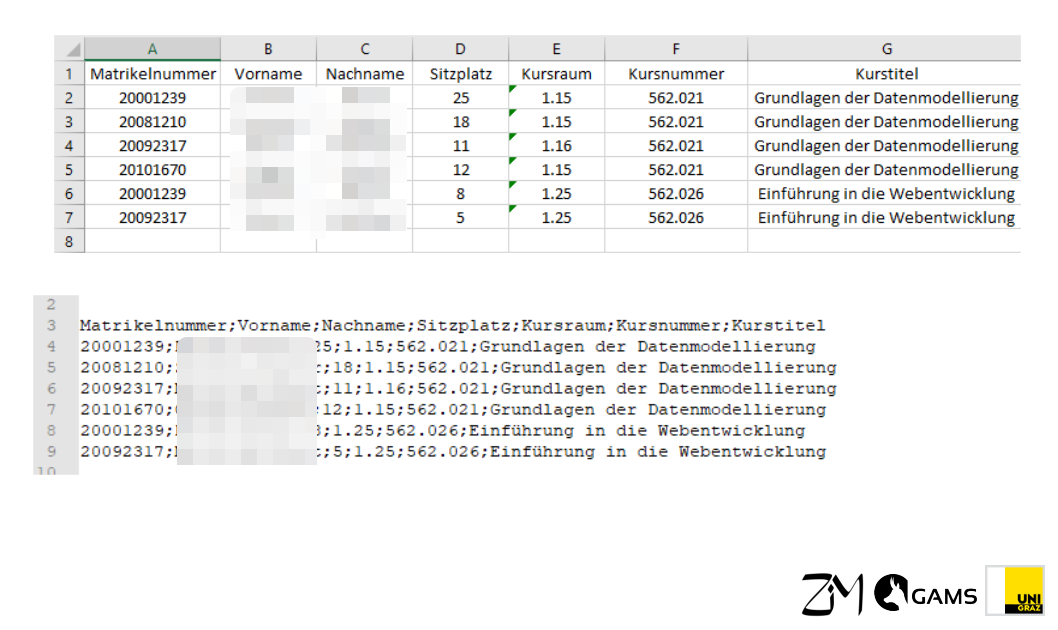
\includegraphics[width=\textwidth]{img/wdh-studierende-csv.png}
\end{frame}

%------------------------------------------------------------------------------
\begin{frame}[allowframebreaks]{Repräsentation von ER-Modellen als Tabellen}
    \begin{itemize}
        \item Entitätsklasse $\to$ Tabelle
        \item Attributklasse $\to$ Spalte
        \begin{itemize}
            \item mehrwertige Attribute $\to$ eigene Tabelle
        \end{itemize}
        \item Relation
            \begin{itemize}
                \item 1:1 $\to$ Schlüssel der einen Entität (Tabelle) wird als Referenz ("foreign key"/"Fremdschlüssel") in der anderen Tabelle eingefügt (eigene Spalte). 
                \item 1:n $\to$ Schlüssel der 1-seitigen Entität (Tabelle) wird als Referenz ("foreign key"/"Fremdschlüssel") in der n-seitigen Tabelle eingefügt (eigene Spalte)
                \item n:m $\to$ eigene Tabelle, die die Schlüssel der beiden Entitäten als Spalten enthält
                \item n-äre Relationen $\to$ eigene Tabelle, die die Schlüssel aller Entitäten als Spalten enthält
                \item Attribute zu Relationen $\to$ eigene Tabelle, die die Schlüssel der beteiligten Entitäten als Spalten und Spalten für die Attribute enthält
                \item mehrwertige Attribute $\to$ eigene Tabelle, die den Schlüssel der Entität als Fremdschlüssel enthält (also wie eine 1:n-Relation modelliert wird) und eine Spalte für das Attribut enthält.
                \item zusammengesetzte Attribute $\to$ eigene Tabelle, die den Schlüssel der Entität als Fremdschlüssel enthält (also wie eine 1:n-Relation modelliert wird) und Spalten für die  Teilattribute enthält.
            \end{itemize}
    \end{itemize}
\end{frame}

%------------------------------------------------------------------------------
\begin{comment}
\begin{frame}[standout]
    \alert{Lektüre}-Zusammenfassung: \\
    Chen, ER-Modelle \\[1em]
    {\footnotesize Bitte \alert{\href{https://docs.google.com/presentation/d/1v_j9Jms21hZokX9hLJ_7kcnV63FJPHTHNowfLVLiYys/edit?usp=sharing}{hier im Google Slides zusammenfassen}}; 1 Person stellt dann vor. \\
    Themen 1 und 2 für jene ohne größere DB-Vorwissen; 3 und 4 bitte möglichst, falls schon gewisses Programmierungs-/DB-Wissen vorhanden ist. \\
    Aufgabe ist nicht, Details herauszupicken -- stark Technisches kann man auch weglassen. \alert{Bitte um Fokus auf die Verständnis-Aspekte.} Man kann gern zur Hilfe andere Materialien dazunehmen. Versuchen, den Mitstudierenden den Text möglichst verständlich aufzubereiten/zusammenzufassen. \\
    Zeit ca. 20min}
\end{frame}
\end{comment}
%------------------------------------------------------------------------------
\begin{frame}{Vom realweltichen Ding zur relationalen Datenbank?}
    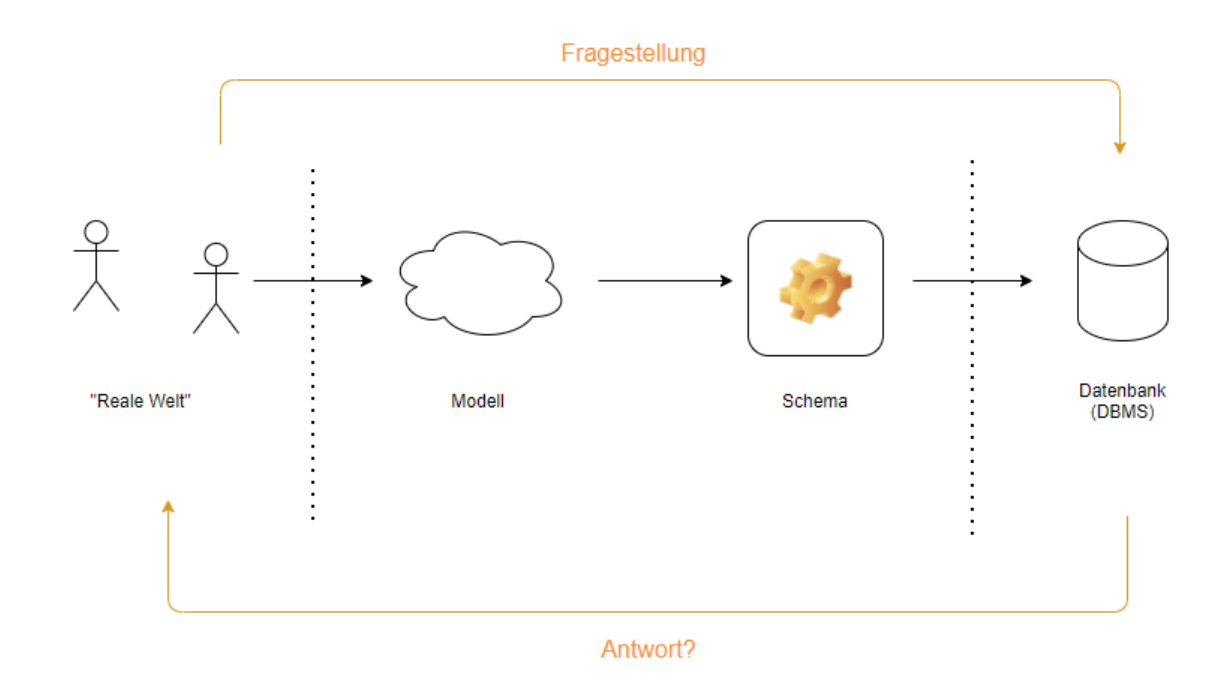
\includegraphics[width=\textwidth]{img/von-welt-zu-db.png}
\end{frame}

%------------------------------------------------------------------------------
\begin{frame}{Der Übergang zur Datenbank}
    % ----------------------------------------------
  \begin{columns}[T,onlytextwidth]
  \metroset{block=fill}
    \column{0.4\textwidth}\footnotesize
    \begin{block}{Datenanalyse Bsp: Tabelle aus Orten}
    \begin{itemize}
        \item Sind die Koordinatenpaare in der Tabelle einzigartig (oder gibt es Dopplungen)?
        \item Gruppiere und zähle die Orte nach Anzahl der Nachkommastellen des Längengrades etc. 
        \item Was gibt es für Abfragen an Visualisierungsmöglichkeiten?
    \end{itemize}
    \end{block}

    % ----------------------------------------------

    \column{0.55\textwidth}
      \metroset{block=fill}
      \begin{exampleblock}{Vorschau: Themenblock relationale Datenbanken}
      \begin{enumerate}\small
          \item  \textbf{Informations- und Datenmodellierung} = Der Weg in die Datenbank
          \item \textbf{Datenanalyse} = Informationen aus der Datenbank wieder herausholen, um Fragestellungen zu beantworten / Strukturierte Information repräsentiert durch Daten abfragen
      \end{enumerate} 
      \end{exampleblock}
  \end{columns}
\end{frame}

%------------------------------------------------------------------------------
\begin{comment}
\begin{frame}[standout]
    \alert{Lektüre} auf nächste Einheit: \\
    McCarty, Modelling
\end{frame}
\end{comment}

%------------------------------------------------------------------------------
\begin{frame}[standout]
    \alert{Hausübung:} Installation von \alert{\href{https://sqlitebrowser.org/dl/}{SQLite}} \\[1em]
    {\footnotesize
    \begin{enumerate}
        \item ggf. in Gruppen zusammenfinden nach Betriebssystem (Linux, Windows, Mac)
        \item wer es schon hat, kann gehen
        \item von mir aus braucht man nicht den Browser, sondern nur SQLite 
        \item wer es noch nicht hat, jetzt geht und dann doch Probleme hat, muss es sich selbst organisieren
        \item $\to$ Möglichkeit bei der Installation Hilfe zu bekommen, falls was nicht klappt
        \item \alert{Tutorials: \href{https://www.tutorialspoint.com/sqlite/sqlite_installation.htm}{Tutorialspoint} | \href{https://www.sqlitetutorial.net/download-install-sqlite/}{SQLiteTutorial} | \href{https://github.com/sqlitebrowser/sqlitebrowser}{SQLiteBrowser Github}}
    \end{enumerate}
    }
\end{frame}
